\documentclass{elegantbook}

\definecolor{LightGray}{gray}{0.9}
\newcommand{\CN}{BIOS 7300\\[0.5cm] Survival Data Analysis}
\newcommand{\Ti}{Homework 6}
\newcommand{\Pf}{Dr.\ Tang}
\newcommand{\FN}{Zehao}
\newcommand{\LN}{Wang}
\usepackage[fontsize=14pt]{fontsize}

\usepackage{longtable}

\usepackage{minted}

\usepackage{enumitem}
\renewcommand{\chaptername}{Homework}
\begin{document} 
\begin{titlepage}
    \begin{center}    
    
\includegraphics[width=0.6\textwidth]{Tulane.png}\\[1cm]    
    
    \textsc{\Huge \CN}\\[0.5cm]
    \textsc{\large \Pf}\\[1.0cm]
    
    \textsc{\LARGE \Ti}\\[0.5cm]
    \textsc{\large \LN, \FN}\\
    {Master student in Statistics of Math Dept.}
    
    % Author and supervisor
    
    \vfill
    
    % Bottom of the page
    {\Large \emph{\today}}
    
    \end{center}
\end{titlepage}

\thispagestyle{empty}
\tableofcontents
\setcounter{chapter}{5}
\chapter{}

\begin{exercise*}[1]
    Use the data ``Smoke'', with age, treat and employment as predictors. We treat age as a variate and treat and employment as factors. In addition to the main effects, we also consider the interaction between treat and employment. So the model is ``survival time $\sim$ age treat | employment''. Based on the model, answer the following questions: 
    \begin{enumerate}[a)]
        \item Estimate the survival functions for an individual with treat=`0', age 50, and full time employed (employment = “ft”).\label{q1pa}
        \item Based on the estimate in part~\ref{q1pa}, estimate the median survival time for an individual with treat=`0', age 50, and full time employed (employment = “ft”). 
        \item Estimate the risk adjusted survivor function for the whole sample by averaging the individual estimated survival curves. 
        \item Are there significant differences in survival times between subjects with age 50, treat=`1', and employment = “pt” and subjects with age 50, treat=`0', and employment = “pt”? 
        \item Are there significant differences in survival times between subjects with age 50, treat=`1', and employment = “pt” and subjects with age 45, treat=`0', and employment = “ft”?
        \item Among subjects with treat = `0', are there significant differences in survival times across the different employment groups? 
    \end{enumerate}
\end{exercise*}

\begin{solution}
    \begin{enumerate}[(a)]
        \item \begin{minted}[frame=lines,
            framesep=2mm,
            baselinestretch=1.2,
            bgcolor=LightGray,
            fontsize=\footnotesize]{SAS}
DATA HW6_1; 
SET "Z:\Documents\GitHub\MS-Stat-Tulane
\Survival Data Analysis\HW06\smoke.sas7bdat"; 
PROC PHREG DATA = HW6_1;
CLASS treat (ref = "0") employment (ref = "ft");
MODEL time*status(0)=age treat | employment;
BASELINE out=a survival=s lower=lcl upper=ucl CUMHAZ=cmh;
RUN; 
        \end{minted}
        \begin{figure}[H]
            \centering
            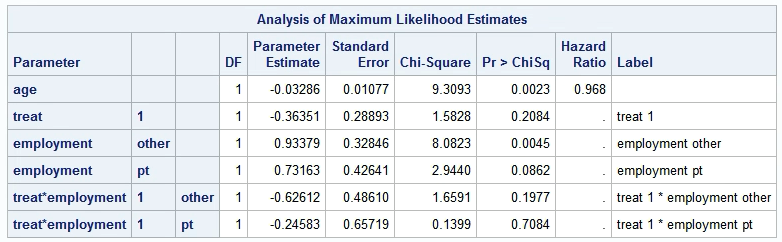
\includegraphics[width = .7\textwidth]{HW6_1.png}
        \end{figure}
        \[h(t)=h_0(t)e^{a X_{age}+b X_{treat_1}+c_1 X_{other}+c_2 X_{pt} + d_1X_{other}X_{treat_1}+ d_2X_{pt}X_{treat_1}}\]
        \[S_1(t)=S_0(t)^{\exp(-0.03286\times(50-48.84))}=S_0(t)^{0.9626}. \]
        \item \begin{minted}[frame=lines,
            framesep=2mm,
            baselinestretch=1.2,
            bgcolor=LightGray,
            fontsize=\footnotesize]{SAS}
PROC PRINT DATA = a; 
RUN; 
        \end{minted}
        \begin{footnotesize}
            \begin{longtable}[c]{lllllllll}
                \hline
                \textbf{Obs} & \textbf{age} & \textbf{treat} & \textbf{employment} & \textbf{time} & \textbf{s} & \textbf{lcl} & \textbf{ucl} & \textbf{cmh} \\ \hline
                \endfirsthead
                %
                \endhead
                %
                \hline
                \endfoot
                %
                \endlastfoot
                %
                \textbf{1}  & 48.84 & 0 & ft & 0   & 1       & .       & .       & 0       \\
                \textbf{2}  & 48.84 & 0 & ft & 0   & 0.92775 & 0.88155 & 0.97636 & 0.075   \\
                \textbf{3}  & 48.84 & 0 & ft & 1   & 0.89447 & 0.83617 & 0.95684 & 0.11153 \\
                \textbf{4}  & 48.84 & 0 & ft & 2   & 0.85271 & 0.78123 & 0.93073 & 0.15933 \\
                \textbf{5}  & 48.84 & 0 & ft & 3   & 0.84546 & 0.77186 & 0.92608 & 0.16787 \\
                \textbf{6}  & 48.84 & 0 & ft & 4   & 0.82381 & 0.7442  & 0.91194 & 0.19382 \\
                \textbf{7}  & 48.84 & 0 & ft & 5   & 0.80921 & 0.72573 & 0.90228 & 0.2117  \\
                \textbf{8}  & 48.84 & 0 & ft & 6   & 0.80183 & 0.7165  & 0.89733 & 0.22085 \\
                \textbf{9}  & 48.84 & 0 & ft & 7   & 0.79448 & 0.70733 & 0.89237 & 0.23007 \\
                \textbf{10} & 48.84 & 0 & ft & 8   & 0.77222 & 0.6799  & 0.87707 & 0.25849 \\
                \textbf{11} & 48.84 & 0 & ft & 10  & 0.76458 & 0.6706  & 0.87173 & 0.26843 \\
                \textbf{12} & 48.84 & 0 & ft & 12  & 0.74941 & 0.65228 & 0.86101 & 0.28846 \\
                \textbf{13} & 48.84 & 0 & ft & 14  & 0.69736 & 0.5909  & 0.82301 & 0.36045 \\
                \textbf{14} & 48.84 & 0 & ft & 15  & 0.66637 & 0.55502 & 0.80005 & 0.40592 \\
                \textbf{15} & 48.84 & 0 & ft & 16  & 0.65841 & 0.54592 & 0.7941  & 0.41792 \\
                \textbf{16} & 48.84 & 0 & ft & 20  & 0.6505  & 0.53691 & 0.78813 & 0.43001 \\
                \textbf{17} & 48.84 & 0 & ft & 21  & 0.63487 & 0.51926 & 0.77621 & 0.45434 \\
                \textbf{18} & 48.84 & 0 & ft & 25  & 0.62677 & 0.51023 & 0.76994 & 0.46718 \\
                \textbf{19} & 48.84 & 0 & ft & 28  & 0.60203 & 0.48305 & 0.75031 & 0.50745 \\
                \textbf{20} & 48.84 & 0 & ft & 30  & 0.57705 & 0.45584 & 0.73049 & 0.54983 \\
                \textbf{21} & 48.84 & 0 & ft & 40  & 0.56855 & 0.4467  & 0.72364 & 0.56467 \\
                \textbf{22} & 48.84 & 0 & ft & 42  & 0.56    & 0.43752 & 0.71675 & 0.57983 \\
                \textbf{23} & 48.84 & 0 & ft & 45  & 0.55145 & 0.42842 & 0.7098  & 0.5952  \\
                \textbf{24} & 48.84 & 0 & ft & 49  & 0.54297 & 0.41943 & 0.70289 & 0.61071 \\
                \textbf{25} & 48.84 & 0 & ft & 50  & 0.53437 & 0.41037 & 0.69584 & 0.62666 \\
                \textbf{26} & 48.84 & 0 & ft & 56  & 0.49255 & 0.36731 & 0.66049 & 0.70816 \\
                \textbf{27} & 48.84 & 0 & ft & 60  & 0.47459 & 0.34915 & 0.6451  & 0.74531 \\
                \textbf{28} & 48.84 & 0 & ft & 63  & 0.45667 & 0.33135 & 0.62937 & 0.7838  \\
                \textbf{29} & 48.84 & 0 & ft & 65  & 0.44755 & 0.32244 & 0.62122 & 0.80396 \\
                \textbf{30} & 48.84 & 0 & ft & 75  & 0.4385  & 0.31365 & 0.61303 & 0.82441 \\
                \textbf{31} & 48.84 & 0 & ft & 77  & 0.42066 & 0.29657 & 0.59667 & 0.86593 \\
                \textbf{32} & 48.84 & 0 & ft & 80  & 0.41169 & 0.28804 & 0.58843 & 0.88748 \\
                \textbf{33} & 48.84 & 0 & ft & 84  & 0.4026  & 0.27941 & 0.5801  & 0.90981 \\
                \textbf{34} & 48.84 & 0 & ft & 100 & 0.39342 & 0.27072 & 0.57172 & 0.93288 \\
                \textbf{35} & 48.84 & 0 & ft & 105 & 0.3843  & 0.26214 & 0.56339 & 0.95632 \\
                \textbf{36} & 48.84 & 0 & ft & 110 & 0.37486 & 0.25336 & 0.55464 & 0.9812  \\
                \textbf{37} & 48.84 & 0 & ft & 140 & 0.33855 & 0.2205  & 0.51981 & 1.08307 \\
                \textbf{38} & 48.84 & 0 & ft & 155 & 0.32912 & 0.21213 & 0.51062 & 1.11134 \\
                \textbf{39} & 48.84 & 0 & ft & 170 & 0.30993 & 0.19542 & 0.49156 & 1.17139 \\ \hline
                \end{longtable}
        \end{footnotesize}
        
        \[S_1(t)=0.5\Rightarrow S_0(t)=e^{\frac{\ln(0.5)}{0.9626}}=0.48671. \]
        So, median time is 60. 
        \item \begin{minted}[frame=lines,
            framesep=2mm,
            baselinestretch=1.2,
            bgcolor=LightGray,
            fontsize=\footnotesize]{SAS}
proc sort data=a;by time;run;
proc means data=a;by time;var s;output out=aa;run;
proc lifetest data=HW6_1 outsurv=c;
time time*status(0) ;
run;
data dd;merge aa c;by time;run;
proc gplot data=dd;
plot SURVIVAL*time s*time / overlay;
symbol1 interpol=stepJ value=dot color=red;
symbol2 interpol=stepJ value=c color=blue;
where _STAT_="MEAN";
run;
        \end{minted}
        \begin{figure}[H]
            \centering
            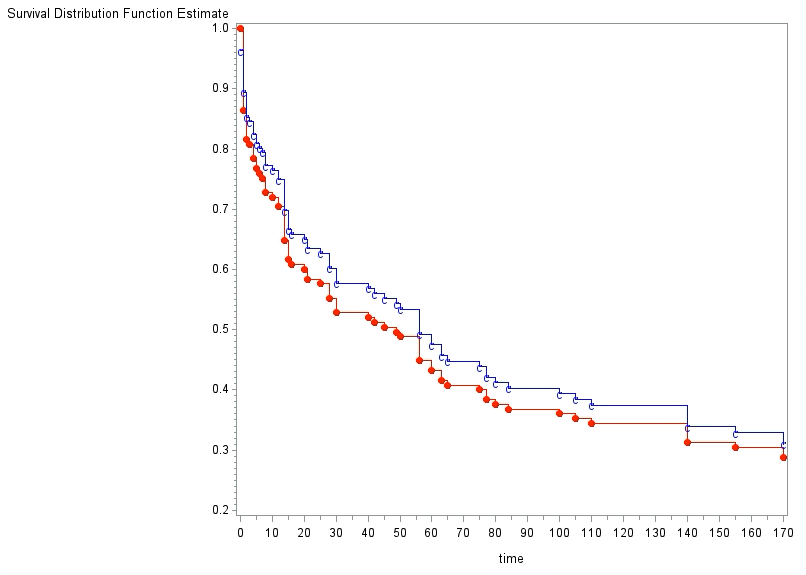
\includegraphics[width=0.8\textwidth]{HW6_2.png}
        \end{figure}
        \item \begin{minted}[frame=lines,
            framesep=2mm,
            baselinestretch=1.2,
            bgcolor=LightGray,
            fontsize=\footnotesize]{SAS}
PROC PHREG DATA = HW6_1;
CLASS treat (ref = "0") employment (ref = "ft");
MODEL time*status(0)=age treat | employment;
CONTRAST "employment"
treat 1 employment 0 0 treat*employment 0 1 age 0/estimate;
run;
        \end{minted}
        \begin{figure}[H]
            \centering
            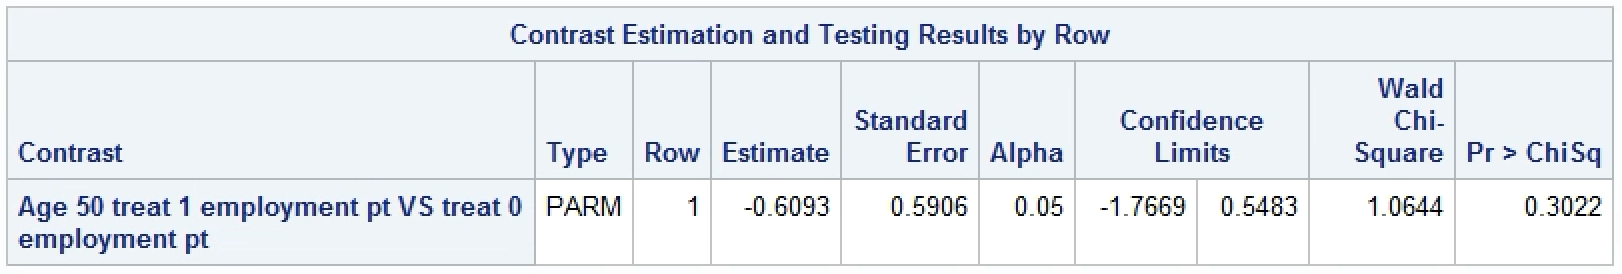
\includegraphics[width=.6\textwidth]{HW6_3.png}
        \end{figure}
        p-value is $0.3>0.05$, so it is not significant.
        \item \begin{minted}[frame=lines,
            framesep=2mm,
            baselinestretch=1.2,
            bgcolor=LightGray,
            fontsize=\footnotesize]{SAS}
PROC PHREG DATA = HW6_1;
CLASS treat (ref = "0") employment (ref = "ft");
MODEL time*status(0)=age treat | employment;
CONTRAST "employment"
treat 1 employment 0 1 treat*employment 0 1 age 5/estimate;
run;
        \end{minted}
        \begin{figure}[H]
            \centering
            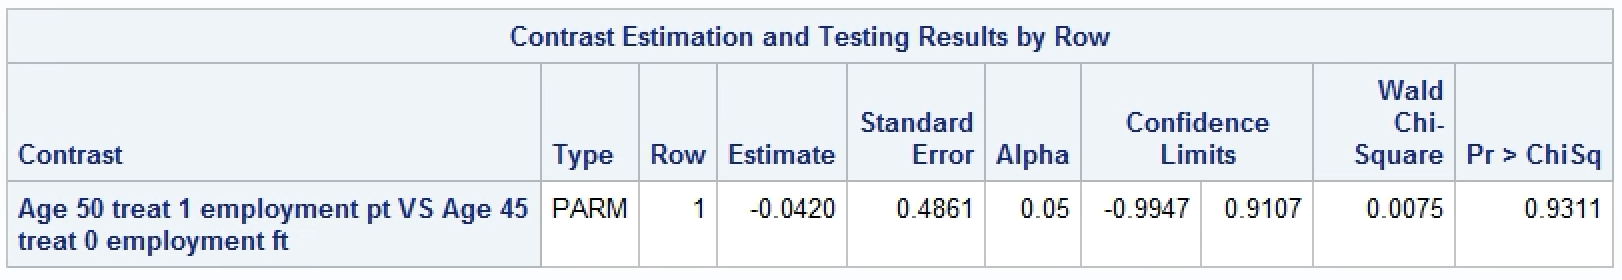
\includegraphics[width=.6\textwidth]{HW6_4.png}
        \end{figure}
        p-value is $0.9311>0.05$, so it is not significant.
        \item \begin{minted}[frame=lines,
            framesep=2mm,
            baselinestretch=1.2,
            bgcolor=LightGray,
            fontsize=\footnotesize]{SAS}
PROC PHREG DATA = HW6_1;
CLASS treat (ref = "0") employment (ref = "ft");
MODEL time*status(0)=age treat | employment;
CONTRAST "employment"
treat 0 employment -1 1,  employment 1 0, employment 0, 1/estimate;
run;
        \end{minted}
        \begin{figure}[H]
            \centering
            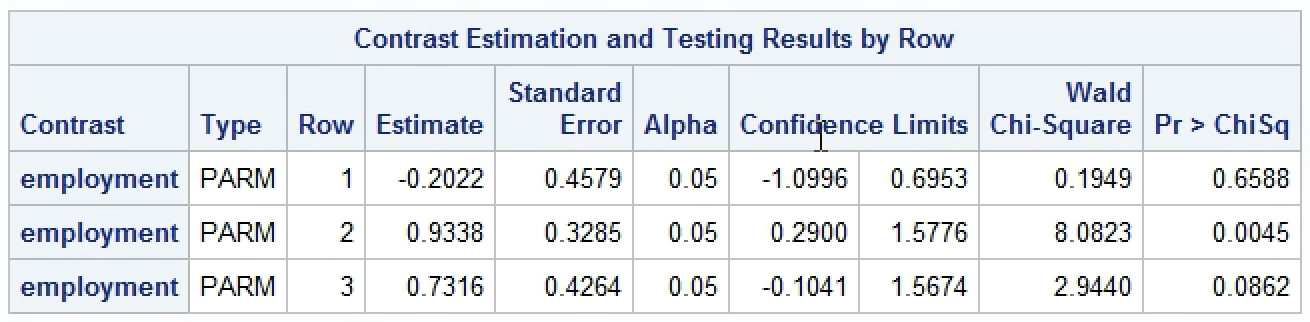
\includegraphics[width=.6\textwidth]{HW6_5.png}
        \end{figure}
        From p-value, we can see that only ft VS other is significant. 
    \end{enumerate}
\end{solution}

\begin{exercise*}[2]
    In a survival data analysis on the survival time of some patients, we are interested in how age, gender, disease severity and living status are related with the survival outcomes. We applied the following SAS program to the data.
    \begin{minted}[frame=lines,
        framesep=2mm,
        baselinestretch=1.2,
        bgcolor=LightGray,
        fontsize=\footnotesize]{SAS}
proc phreg;
class gender disease living ;
model time*status(0)=age gender disease|living;
contrast "test 1" disease 1 -1;
contrast "test 2" disease*living 0 0 0 1, disease*living 0 0 0 0 1,
disease*living 0 0 0 0 0 1;
contrast "test 3" disease*living 1, disease*living 0 1,
disease*living 0 0 1, disease*living 0 0 0 1,
disease*living 0 0 0 0 1, disease*living 0 0 0 0 0 1;
contrast "test 4" living 1 disease*living 0 0 0 1,
living 0 1 disease*living 0 0 0 0 1,
living 0 0 1 disease*living 0 0 0 0 0 1;
run;
    \end{minted}
    The SAS output of the program is saved in file “hw6sasoutput.pdf”. Based on the SAS output answer the following questions:

    \begin{enumerate}[a)]
        \item Clearly define the dummy variables in the program and write down the fitted proportional hazards model. 
        \item Are there significant interactions between disease and living status? 
        \item What does the test (“test 1”) test? Explain it in terms of hazard ratios among different subpopulations. 
        \item What do the tests (“test 2” --- “test 4”) test? 
    \end{enumerate}
\end{exercise*}

\begin{solution}
    \begin{enumerate}[a)]
        \item \begin{enumerate}[i)]
            \item $Gender = 1$: $X_{Gender} = 1$, $Gender = 2$: $X_{Gender} = 0$. 
            \item $Disease = 1$: $X_{Disease} = 1\ 0$, $Disease = 2$: $X_{Disease} = 0\ 1$, $Disease = 3$: $X_{Disease} = 0\ 0$. 
            \item $Living = 1$: $X_{Living} = 1\ 0\ 0$, $Living = 2$: $X_{Living} = 0\ 1\ 0$, $Living = 3$: $X_{Living} = 0\ 0\ 1$, $Living = 4$: $X_{Living} = 0\ 0\ 0$. 
            \begin{align*}
                h(t)=h_0(t)\exp(&0.00242X_{Age} -0.00721X_{Gender}-0.80027 X_{disease_1}\\
                &-0.34501 X_{disease_2}-6.51011X_{living_1}+0.19590 X_{living_2}\\
                &+1.21877 X_{living_3}+0.40291 X_{disease_1}X_{living_1}\\
                &+1.86452X_{disease_1}X_{living_2}+0.19159 X_{disease_1}X_{living_3}\\
                &+2.18213 X_{disease_2}X_{living_1}+0.66501X_{disease_2}X_{living_2}\\
                &+0.24421 X_{disease_2}X_{living_3})
            \end{align*}
        \end{enumerate}
        \item Yes, p-value for disease*living is $0.0097<0.05$. 
        \item Test if there is a significant difference for survival time between disease 1 and disease 2. For Disease 1, 
        \[h(t)= h_0(t)\exp(-0.80027 X_{disease_1})\]
        For Disease 2, 
        \[h(t)= h_0(t)\exp(-0.34501 X_{disease_2})\]
        And 
        \[HR(test1)=\exp(-0.80027 X_{disease_1}+0.34501 X_{disease_2})\]
        p-value for test1 is $0.4138>0.05$. So it is not significant. 
        \item \begin{enumerate}[i)]
            \item Test 2: If there is a significant difference for disease 2 and all levels of living status.
            \item Test 3: If there is a significant effect for all interactions between living status and disease. 
            \item Test 4: If there is a significant effect for disease 2 among different living status.
        \end{enumerate}
    \end{enumerate}
\end{solution}

\end{document}